\documentclass[a4paper,14pt]{extreport}

\usepackage[T2A]{fontenc}
\usepackage[utf8]{inputenc}
\usepackage{totcount}

\usepackage[english,russian]{babel}

\usepackage{amsthm}

\usepackage{hyperref}

\usepackage[dvips]{graphicx}
\usepackage{caption}
\usepackage{subcaption}
\graphicspath{{images/eps/}}

\usepackage{titlesec}
\usepackage{listings}
\usepackage{indentfirst}
\usepackage{cite}

\usepackage{geometry}
\geometry{left=3cm}
\geometry{right=1cm}
\geometry{top=1.5cm}
\geometry{bottom=2cm}

\renewcommand{\baselinestretch}{1.2}

\lstset{numbers=left,
        frame=single,
        breaklines=true,
        breakatwhitespace=true,
        basicstyle=\ttfamily\small}

\begin{document}

\makeatletter
\renewcommand{\@biblabel}[1]{#1.}
\makeatother

\titleformat{\chapter}[hang]{\huge\bfseries}{\thechapter. }{0pt}{\hyphenpenalty=10000\huge\bfseries}

\renewcommand{\theenumi}{\arabic{enumi}}
\renewcommand{\labelenumi}{\arabic{enumi}}
\renewcommand{\theenumii}{.\arabic{enumii}}
\renewcommand{\labelenumii}{\arabic{enumi}.\arabic{enumii}}
\renewcommand{\theenumiii}{.\arabic{enumiii}}
\renewcommand{\labelenumiii}{\arabic{enumi}.\arabic{enumii}.\arabic{enumiii}}

\newtotcounter{figurecnt}
\def\oldfig{} \let\oldfig=\figure
\def\figure{\stepcounter{figurecnt}\oldfig}
%òàáëèö (only longtable)
\newtotcounter{tablecnt}
\def\oldtab{} \let\oldtab=\table
\def\table{\stepcounter{tablecnt}\oldtab}

\newtotcounter{citeitem}
\renewcommand{\citeform}[1]{%
\ifnum#1>\totvalue{citeitem}%
{\setcounter{citeitem}{#1} }\fi%
#1%
}

\regtotcounter{page}

\def\formbytotal#1#2#3#4#5{%
    \newcount\c
    \c \totvalue{#1}\relax
    \newcount\last
    \newcount\pnul
    \last \c\relax
    \divide \last 10
    \pnul \last\relax
    \divide\pnul 10
    \multiply \pnul-10
    \advance \pnul\last
    \multiply \last-10
    \advance \last\c
    \total{#1}~#2%
    \ifnum\pnul=1#5\else%
        \ifcase\last#5\or#3\or#4\or#4\or#4\else#5\fi
    \fi
}

\renewcommand{\lstlistingname}{Листинг}
\renewcommand\contentsname{Содержание}

\newtheorem{Def}{Определение}[section]

\setcounter{page}{2}

\chapter*{Реферат}

	%TODO: разберись, как пишется: "онлайн среда разработки" - с дефисом или без 
	Дипломный проект изложен на~\formbytotal{page}{страниц}{е}{ах}{ах}, содержит \formbytotal{tablecnt}{таблиц}{у}{ы}{}, \formbytotal{figurecnt}{рисун}{ок}{ка}{ков}, 11 источников.

	Целью данного проекта является создание новой версии онлайн среды разработки для языка Котлин.

	В результате данного проекта было создано интернет-приложение с масштабируемой архитектурой, располагающееся по адресу\\ http://try.kotlinlang.org/. 
	
	Работа состоит из четырёх глав, введения и заключения.
Во введении в краткой форме объясняются причины возникновения необходимости выполнения такого рода работы, цель и задачи проекта.
В первой главе проводится краткий обзор предметной области
Во второй главе описывается устройство приложения.
В третьей главе приведено описание системы публикации приложения с учётом масштабируемой архитектуры.
Четвёртая глава посвящена тестированию приложения.
В заключении подводятся итоги и описываются возможные направления дальнейших работ.

\clearpage

\tableofcontents

\chapter*{Введение}
\addcontentsline{toc}{chapter}{Введение}  

	На ранних этапах развития интернета каждая web-страница доставлялась клиенту как статический документ, а интерактивность достигалась за счёт последовательности различных страниц. У такого подхода был недостаток -- при каждом значительном изменении веб страницы требовалось обратиться к серверу и перезагрузить эту страницу целиком. 

	В 1995 году компания Netscape выпустила язык программирования JavaScript, который исполнялся на стороне клиента и позволял выполнять ряд задач не обращаясь при этом к серверу. Вторым важным моментом было развитие AJAX запросов -- запросов к серверу, которые не требовали перезагрузки страницы. 
	
	Развитие этих двух технологий привело к появлению интернет-приложений -- интерактивных веб сайтов, которые могут целиком располагаться на одной странице,  взаимодействуя с пользователем при помощи JavaScript кода, а с сервером при помощи AJAX запросов. На сегодняшний день такой формат сайтов очень популярен, т.к. он позволяет намного больше, чем последовательность интернет-страниц, например, писать браузерные игры, отображать карту и.т.д.
	
	Одним из многочисленных типов интернет-приложений являются онлайн среды разработки -- сайты, которые позволяют запустить код на том или ином языке в браузере. Они позволяют пользователям познакомиться с новым для них языком, а так же предоставляют простой способ демонстрировать другим пользователям свой код (например, сайт jsfiddle почти всегда используется для публикации кода в качестве иллюстрации к ответам на вопросы, касающиеся HTML/CSS/JavaScript).
	
	Подобные приложения есть почти для всех распространённых языков программирования, например:
\begin{itemize}
	\item http://www.simplyscala.com/ - приложение, позволяющее запускать код на языке scala. 
	\item http://try.ceylon-lang.org/ - приложение, позволяющее запускать код на языке ceylon
	\item http://www.tutorialspoint.com/ - приложение, позволяющее запускать код на большом количестве разнообразных языков программирования
	\item \dots
\end{itemize}


	Онлайн среда разработки для языка Котлин называется Kotlin Web Demo. Данное приложение учитывает специфику  языка и позволяет как запускать код внутри виртуальной машины Java, которая располагается на сервере, так и транслировать код в JavaScript и исполнять его в браузере. Также в этом приложении есть подсветка синтаксиса, подсветка ошибок и автодополнение кода, что значительно упрощает процесс его написания.
	

	Недостатком данной среды разработки является исполнение всех запросов внутри одного сервера. Такая архитектура приложения является самой простой, однако при увеличении нагрузки приложение утрачивает работоспособность. Подобная ситуация наблюдалась при публикации Kotlin Web Demo и может повториться, например, при публикации новой версии Котлина.
	
	
	Вторым существенным недостатком была необходимость размещения  исполняемого кода  пользовательского примера внутри одного файла. Это не было проблемой само по себе, т.к. основная цель - дать пользователю познакомиться с языком, а не предоставить ему возможность писать большие программы, однако это стало проблемой когда возникла идея использовать Kotlin Web Demo для запуска программ-заданий. Каждое такое задание требует от пользователя написать код на Котлине, который решает определённую задачу, а потом при помощи тестов проверяет, что код решает задачу корректно. Для реализации этого требовалось разделить код на файл с тестами и файл с пользовательским кодом, что и привело к возникновению вышеописанной проблемы.
	
	
	\underline{Целью} данного проекта является создание новой версии онлайн среды разработки
	
	Основные \underline{задачи}, решаемые в работе:
	\begin{itemize}
		\item { \bf Создание автоматически масштабируемой архитектуры приложения} -- для работоспособности сервера в случае резкого увеличения нагрузки.
		\item { \bf Поддержка многофайловых проектов и JUnit тестов} -- для запуска программ-заданий
	\end{itemize}
		



\chapter{Обзор предметной области}
\section{Технологии разработки интернет-приложения}
	Данный проект, как и другие интернет-приложения,  состоит из клиентской и серверной части. В этой главе даётся краткий обзор тех технологий и языков программирования, которые использовались для написания обеих частей.
\subsection{Клиентская часть}
	Для написания клиентской части используются следующие технологии и языки программирования:
\begin{itemize}
	\item \textbf{HTML/CSS} -- стандартные технологии веб-программирования, используемые для верстки веб-приложения.
	\item \textbf{JavaScript} -- высокоуровневый динамический язык программирования, который используется в основном для клиентской части интернет-приложений. Позволяет взаимодействовать с пользователем, изменять видимый пользователю документ, отправлять AJAX-запросы серверу. JavaScript позволяет писать как в функциональном, так и в объектно-ориентированном стиле, однако используемое в языке ``прототипное наследование'' обусловливает отличия в работе с объектами по сравнению с традиционными языками, использующими классы.
	\item \textbf{Jquery} -- распространённая библиотека для JavaScript, которая добавляет простой и достаточно удобный интерфейс для отправки запросов к серверу, обработки событий, взаимодействия с DOM-деревом и многого другого.
	\item \textbf{Jquery UI} -- библиотека, основанная на JQuery. Предоставляет интерфейс для создания различных элементов сайта, таких как диалоги, вкладки, кнопки и т.д..
	\item \textbf{CodeMirror} -- редактор кода, написанный на языке JavaScript. Де-факто является стандартом для тех приложений, в которых требуется редактировать/демонстрировать код. На данный момент поддерживает более 100 языков и обладает достаточно простым интерфейсом, позволяющим легко поддержать любой новый язык. Также он обладает системой плагинов, которая позволяет его персонализировать, добавляя те возможности, которые вас интересуют (например, поиск, автодополнение, подсветка текущей строки и.т.д.)
	%TODO: так же и также http://tak-zhe.ru/
	\item \textbf{Котлин} -- статически типизированный объектно-ориентированный язык программирования, который может быть скомпилирован в JavaScript. Котлин, как и JavaScript, позволяет писать не только в объектно-ориентированном, но и в функциональном стиле. Также в Котлине создан ряд абстракций (аннотация native, dynamic тип и др.), которые позволяют взаимодействовать с кодом на JavaScript. Благодаря этому, в большинстве случаев, код, написанный на JavaScript, достаточно легко транслируется в код на Котлине. 
\end{itemize}

\subsection{Сервер}
	Для написания серверной части используются следующие технологии:
\begin{itemize}
\item \textbf{Tomcat} -- сервер, написанный на языке Java и разрабатываемый компанией Apache. Tomcat реализует ряд спецификаций языка Java, таких как Java Servlet и JavaServer Pages. Для обработки запросов, приходящих на сервер, томкат использует отдельные потоки, количество которых может регулироваться в настройках сервера.
\item \textbf{OAuth} -- протокол авторизации. Использование данного протокола позволяет пользователям авторизироваться в различных местах используя, например, свой аккаунт в google, при этом не передавая третьим лицам приватные данные, связанные с данным аккаунтом.
\item \textbf{HTTP session} -- механизм идентификации пользователя между парами ``запрос-ответ''.
\item \textbf{MySql} -- реляционная база данных.
\end{itemize}
 
	
	Также в серверной части приложения используется:
	
\section{Технологии тестирования интернет-приложения}
	%TODO: очень много "тестирования"
	Тестирование интернет-приложения, как правило, состоит из нескольких частей -- тестирования клиентского кода, тестирование серверного кода, а так же тестирование поведения сервера при большом количестве запросов (нагрузочное тестирование).
	
	Для проведения этих частей тестирования в данном проекте используются следующие технологии:
	\begin{itemize}
\item Тестирование серверного кода:
	\begin{itemize}
		\item \textbf{JUnit} -- распространённая библиотека для написания unit-тестов на языке Java.
	\end{itemize}
\item Нагрузочное тестирование:
	\begin{itemize}
		\item \textbf{JMeter} -- графическое Java приложение, предназначенное для написания нагрузочного тестирования и измерения производительности при нагрузочном тестировании. Данное приложение позволяет отправлять различного рода запросы (нас интересуют HTTP запросы) и анализировать производительность сервера при обработке этих запросов.
	\end{itemize}
\item Тестирование клиентского кода:
\begin{itemize}
	\item \textbf{nodejs} -- платформа, позволяющая запускать код на языке JavaScript. Обычно используется для создания серверов и сетевых приложений. В данном проекте используется для запуска karma.
	\item \textbf{karma} -- приложение для запуска тестов на языке JavaScript. Может исполнять тесты во всех популярных браузерах(Google Chrome, Opera, Safari \dots), а так же внутри phantomjs. Это приложение само написано на JavaScript и предназначено для запуска при помощи nodejs.
	\item \textbf{phantomjs} -- браузер без графического интерфейса, созданный для автоматического тестирования веб-приложений. Данный браузер основан на платформе WebKit, что делает его похожим по поведению на такие браузеры, как Chrome и Safari.
	\item \textbf{qunit} -- распространённая библиотека для написания unit-тестов на языке JavaScript.
\end{itemize}
\end{itemize}

\section{Технологии публикации интернет-приложения}
В данной главе освещаются технологии, используемые нами для публикации приложения.
\subsection{Amazon Web Services}
	%TODO: предоставляемый предоставляет
	Amazon Web Service -- это набор сервисов, предоставляемый компанией Amazon. Данные сервисы предоставляют возможность создания масштабируемой инфраструктуры на машинном уровне и состоят из следующих компонент:
\begin{itemize}
	\item \textbf{Amazon EC2 instance} -- пожалуй, один из основных элементов всей инфраструктуры. EC2 instance -- это компьютер, предоставляемый амазоном, параметры которого можно выбирать при старте, основываясь на требованиях к данному компьютеру. В зависимости от параметров меняется и стоимость данного компьютера.
	\item \textbf{Amazon Machine Image (AMI)} -- снимок памяти компьютера, необходим для того, чтобы запустить EC2 instance. Существует большое количество публичных AMI, которые, как правило, содержат операционную систему (например, для запуска EC2 instance с Ubuntu необходимо найти идентификатор AMI содержащего Ubuntu  и указать его при старте машины). Также пользователь может создать свой AMI, содержащий специфичную для данной задачи информацию.
	\item \textbf{Launch Configuration} -- конфигурация, которая содержит все данные, необходимые для запуска EC2 instance, такие как: 
	\begin{itemize}
		\item Instance type -- определяет мощность CPU, количество памяти и другие подобные параметры  EC2 instance.
		\item AMI ID -- идентификатор AMI.
		\item User Data -- скрипт, который будет исполнен после запуска машины. Позволяет автоматизировать запуск машины.
		\item ...
	\end{itemize}
	\item \textbf{Cloud Watch Monitoring} -- сервис, который собирает и хранит информацию о других сервисах, например, для каждого EC2 instance хранятся: 
	\begin{itemize}
		\item Потребление CPU
		\item Количество операций чтения/записи на диск
		\item \dots
	\end{itemize}
	Вся эта информация доступна через веб интерфейс Amazon. %ссылка на какую-нибудь картинку%.
	\item \textbf{Cloud Watch Monitoring Alarm} -- настраиваемые события внутри Cloud Watch Monitoring. Например, ``среднее потребление CPU у EC2 instnance более 80\% в течении 5 минут''. Может использоваться как для оповещения администратора, так и для управления масштабированием.
	\item \textbf{Auto Scaling Group (ASG)} -- система, позволяющая запускать заданное количество EC2 instance. Их количество может выставляться как вручную, так и на основании Cloud Watch Monitoring Alarmsdamnaleto-ов.
	\item \textbf{Elastic Load Balancer (ELB)} -- балансировщик нагрузки. Распределяет приходящие на него HTTP-запросы между компьютерами, которые к нему подключены.
\end{itemize}


Кроме перечисленных выше сервисов нами использовались сервисы, связанные с безопасностью, доменными именами и.т.д., однако они являются техническими и их описание не представляет особого интереса.

\subsection{Cхема работы автоматического масштабирования в AWS}
	%TODO: "автоматическое масштабирование"
	Перечисленные выше сервисы, как правило, не используются сами по себе, а собираются в большую систему. В данном параграфе я покажу как в общем из описанных выше сервисов получается автоматически масштабируемая система.
	
	Схема работы автоматического масштабирования приведена на рис.\ref{fig:aws_autoscaling}.
	
\begin{figure}[h]
    \centering
    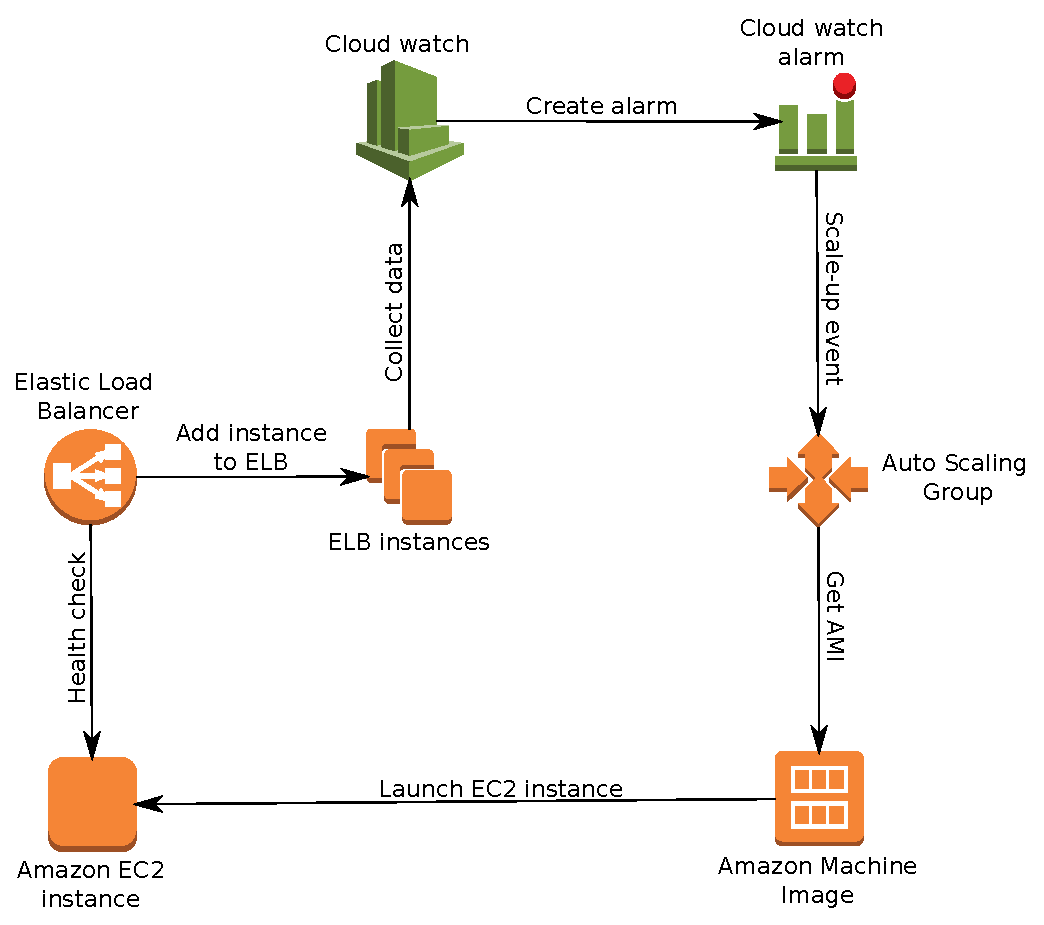
\includegraphics[scale=0.8]{amazon_scale_up.eps} 
    \caption{Принципиальная схема работы автоматического масштабирования в AWS}
    \label{fig:aws_autoscaling}
\end{figure}
	Рассмотрим как это всё работает, начиная с процесса создания. Первым создаётся балансировщик нагрузки (ELB). В начале к нему не прикреплен ни один компьютер, поэтому, если на него приходит запрос, то он просто отвечает HTTP статусом 503 (сервис недоступен).
	
	Далее создаётся система автоматического масштабирования (ASG). При её создании необходимо иметь конфигурацию (Launch Configuration), основываясь на которой она будет запускать новые компьютеры в случае надобности. Также нужно создать события (Cloud Watch Alarms), которые будут послать сигналы для увеличения/уменьшения количества машин в системе масштабирования. Каждое из этих событий следит за потреблением одного из ресурсов, например, CPU и позволяет отреагировать на то, что мы данный ресурс исчерпываем (нужно запустить больше машин), либо у нас его слишком много (нужно остановить несколько машин).
	
	После создания система, используя заданную конфигурацию, автоматически поднимает минимальное количество машин (параметр, передающийся при запуске) и подключает их к ELB. Балансировщик нагрузки выполняет проверку того, что переданные ему машины работоспособны (определённым образом отвечают на определённый запрос) и, как только убеждается в их работоспособности, начинает отправлять туда запросы.
	
	Дальнейшее масштабирование происходит на основе данных в системе мониторинга (Cloud Watch Monitoring). Данные, полученные с запущенных машин, сравниваются с настроенными нами событиями и на основании их система масштабирования автоматически  запускает (аналогично предыдущему пункту), либо останавливает компьютеры.
	
	Кроме описанного выше случая компьютер может быть остановлен, если он в какой-то момент не пройдёт проверку работоспособности от ELB. В такой ситуации система масштабирования попытается поднять новую машину на замену неработоспособной. Это позволяет автоматически восстанавливать систему, если что-то произошло на одном из компьютеров, однако может привести к неприятным последствиям, которые будут освещены в главе \ref{}.

\subsection{Docker}

	Docker - технология виртуализации, которая в последнее время набирает всё большую популярность среди разработчиков. 
	
	Отличие докера от виртуальных машин, которые так же являются способом виртуализации, заключается в основном в легковесности. Каждая виртуальная машина должна кроме приложения (которое может иметь размер в несколько мегабайт) подгружать ещё и окружение (которое может иметь размер в несколько гигабайт). В отличии от этого докер-контейнер содержит только приложение и его зависимости и запускается в изолированном процессе в пространстве пользователя, разделяя ядро с другими контейнерами.
\begin{figure}[h]
	\centering
	\begin{subfigure}[b]{.5\textwidth}
  		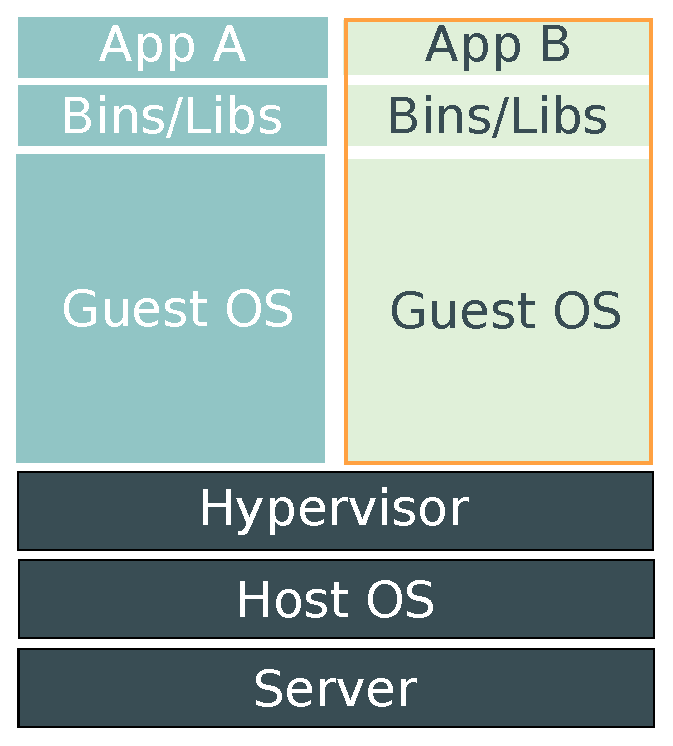
\includegraphics[width=.9\linewidth]{vm_scheme}
  		\caption{Virtual Machines}
  		\label{fig:sub1}
	\end{subfigure}%
	\begin{subfigure}[b]{.5\textwidth}
  		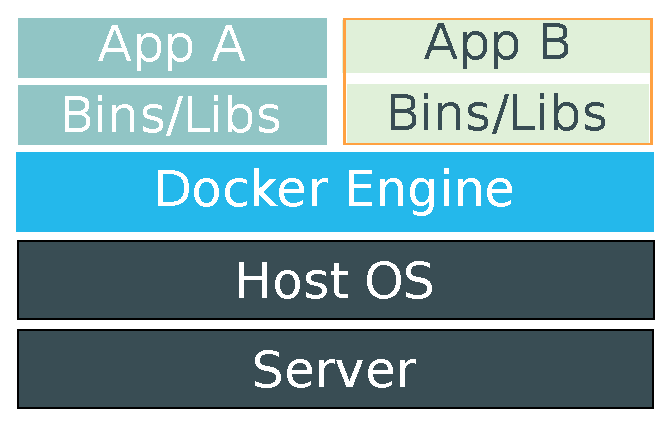
\includegraphics[width=.9\linewidth]{docker_scheme}
  		\caption{Docker}
  		\label{fig:sub2}
	\end{subfigure}
	\caption{Сравнение виртуализации при помощи виртуальных машин и при помощи докер контейнеров}
	\label{fig:test}
\end{figure}

	%TODO: в определениях тире ставить между подлежащим и сказуемым
	Каждый докер-контейнер основан докер-образе. Докер-образ -- это шаблон, по которому мы можем запускать контейнеры. В нём можно указать операционную систему, которую нужно использовать, установить необходимое окружение, и.т.д. Образы можно как собирать, основываясь на файле с инструкциями, так и скачивать с хранилищ.
	
	Каждый образ состоит из слоёв. Слой -- это состояние контейнера после того, как мы выполнили очередную команду. Такая структура позволяет нам при обновлениях образа вместо обновления всего приложения обновить только изменившиеся слои.
\subsection{Операционная система}
\begin{itemize}

	\item {\bf CoreOS} - операционная система, предназначенная для запуска всего внутри контейнеров Linux, например, при помощи докера, о котором шла речь в предыдущем пункте. В связи с такой специфической направленностью в CoreOS отсутствуют почти все привычные для пользователя Linux пакеты и программы (yum, apt-get, wget \dots), грубо говоря, там есть только докер.
	
	\item {\bf systemd} - демон инициализации других демонов в Linux. Systemd позволяет описывать сервис, который мы собираемся запустить, в текстовом виде. Ниже приведён пример файла сервиса, который запускает докер контейнер.
\begin{lstlisting}
[Unit]
Description=My Service
Requires=docker.service
After=docker.service

[Service]	
ExecStart=/usr/bin/docker run busybox /bin/sh -c "while true; do echo Hello World; sleep 1; done"

[Install]
WantedBy=multi-user.target
\end{lstlisting}
\end{itemize}
	Кроме запуска systemd следит за работоспособностью запущенных сервисов и, если какой-то из них возвращает ошибку, перезапускает его (если не настроить обратное).
\section{Подходы к обновлению интернет-приложения}
Существует множество различных способов обновления интернет-приложения в зависимости от требований к нему. Самыми простыми из них являются:
\begin{itemize}
	\item {\bf Выключать приложение для обновления.} Данный подход является наиболее простым, однако обладает рядом очевидных недостатков, а именно:
	\begin{itemize}
		\item Приложение недоступно в течение обновления.
		\item Невозможно протестировать обновлённое приложение перед его публикацией.
		\item Сложно восстановить работоспособность приложения при неудачном обновлении.
	\end{itemize}
	\item {\bf Создавать копию приложения вместе с инфраструктурой.} При таком подходе обновляется то приложение, которое на данный момент не принимает запросы от пользователя. После обновления все запросы начинают отправляться на новую версию приложения, а старая версия становится неактивной до следующего обновления. Недостатком такого подхода является необходимость создания копии всей инфраструктуры.
	\item {\bf Создавать копию приложения (Blue-Green deployment).} Данный подход аналогичен предыдущему, но в нём неактивное приложение располагается внутри той же инфраструктуры, что и активное. Недостатки данного подхода будут описаны подробней в главе \ref{sec}
	%TODO: точку в конце поставь.
	%TODO: вместо номеров много чего у меня ??
\end{itemize}
\chapter{Устройство приложения}
Моё приложение состоит из серверной и клиентской части. Серверная часть в свою очередь состоит из фронтенд сервера - приложения, которое принимает запросы от пользователя и бэкенд серверов, которые обрабатывают ряд запросов, пришедших на фронтенд сервер.


	
	%Написать про базу данных
	%Добавить картинку
	%Обновление бэкенда при обновлении версии Котлина
	%Сказать про JS конфигурацию
\section{Серверная часть}
\subsection{Технологии}
	Для написания серверной части используются следующие технологии:
\begin{itemize}
	\item \textbf{Tomcat} -- сервер, написанный на языке Java и разрабатываемый компанией Apache. Томкат реализует ряд спецификаций языка Java, таких как Java Servlet и JavaServer Pages. Для обработки запросов, приходящих на сервер, томкат использует отдельные потоки, количество которых может регулироваться в настройках сервера. 
	
	Используется как на фронтенд сервере, так и на бэкенд серверах.
	\item \textbf{MySql} -- реляционная база данных. 
	
	Используется в нашем приложении для хранения сохранённых пользовательских проектов.
\end{itemize}


\subsection{Фронтенд сервер}
	Фронтенд сервер принимает все запросы, приходящие от пользователя. Эти запросы делятся на несколько типов:
\begin{itemize}
	\item Запросы, связанные с Котлином (исполнение, подсветка синтаксиса, автодополнение, конвертация из Java, конвертация в JS)
	\item Запросы  к базе данных (добавить/модифицировать/сохранить/удалить проект/файл)
	\item Запросы к фронтенд серверу (выдать код примера, запросы авторизации)
\end{itemize}

	Все запросы связанные с Котлином пересылаются бэкенд серверам, после чего в течении определённого времени ожидается ответ, который отправляется обратно пользователю. Если же ответ не приходит, то пользователю отправляется соответствующее сообщение об ошибке.
	
	Запросы к базе данных отправляются только для авторизированных пользователей, у которых в базе дынных хранятся их программы. Авторизироваться на данный момент можно используя свой аккаунт google, facebook, twitter, github или JetBrains account. В большинстве случаев для авторизации используется протокол OAuth. После того как пользователь авторизировался, его данные (идентификатор, имя, фамилия) записываются внутрь HTTP сессии. 

\subsection{Бэкнед сервер}
	Каждый бэкенд сервер, так же как и фронтенд сервера, представляет собой приложение, запущенное внутри tomcat. 
	
	В качестве библиотеки к данному приложению подключена релизная версия всех библиотек Котлина (runtime, compiler, plugin). Эти библиотеки используются для обработки всех пользовательских запросов.
	
	На данный момент вся обработка запроса, кроме исполнения скомпилированной в java программы, осуществляется в потоке сервера. Это приводит к тому, что мы не можем гарантированно ограничить время исполнения запроса, т.к. поток нельзя завершить извне.
	
	При обработке запроса на исполнение сначала код на языке Котлин компилируется в байткод java. Далее скомпилированный код исполняется в отдельном процессе внутри класса - обёртки. Этот класс выбирается в зависимости от конфигурации проекта, отправленного нам на исполнение.
	
	В случае JVM конфигурации этот класс, используя reflection, запускает функцию main в пользовательском коде, т.е. по большому счёту, просто исполняет пользовательскую программу. При этом весь вывод программы (stdOut, stdErr) перенаправляется в форматированном виде в один поток. Если внутри пользовательского кода вылетает ошибка, она ловится классом обёрткой. По завершению пользовательской программы весь вывод, а так же вылетевшая ошибка (если есть), сериализуются в формат JSON и полученная строчка выводится в stdout класса - обёртки.
	
	В случае Junit конфигурации, используя встроенные средства этой библиотеки, запускаются все тестовые методы, найденные внутри пользовательских классов. При запуске каждого теста сохраняется вывод программы и ошибки, вылетевшие в процессе исполнения. По завершению исполнения всех тестов эта информация так же сериализуется в формат JSON и выводится в стандратный поток вывода.
	
	Процесс, в котором исполняется пользовательская программа, ограничен по памяти (Xmx настройка java-машины), ограничен по времени исполнения (через 5 секунд процесс завершается из сервера), а так же ему запрещён доступ к сети, файловой системе и.т.д. при помощи Java security manager.
	
	
	

\chapter{Инфраструктура}

Для публикации приложения используются Amazon Web Services (AWS) - набор сервисов компании Amazon.

\section{Бэкенд инстансы}
\subsection{Старт новой машины}
	При автоматическом запуске машины мы можем передать очень маленькое количество информации, а именно, идентификатор AMI и User Data - небольшой набор инструкций, который будет выполнен после запуска чистой машины. В данной секции я расскажу о том, как при помощи этого небольшого количества данных можно запускать приложения.
	
	Для того, чтобы запустить чистую машину нам достаточно идентификатора AMI. Первоначально нами был выбран образ с CoreOS, т.к. планировалось запускать приложение внутри докер контейнера, а CoreOS как раз предназначена для таких случаев.
	
	После того как мы запустили чистую машину нам необходимо скачать наше приложение и всю необходимую инфраструктуру используя при этом только докер, т.к. в CoreOS кроме него больше ничего нет.
	
	Теоретически, всё приложение вместе с инфраструктурой можно было бы поместить внутрь одного докер образа, а при старте машины выполнить docker pull. Проблема такого подхода заключается в том, что при обновлении исходного кода приложения, что происходит очень часто, нам приходилось бы добавлять слой, что приводило бы к сильному росту размера образа. Так же при таком подходе нам не удалось бы обновить приложение не убивая докер контейнер, что привело бы к длительным перерывам в работе приложения при его обновлении.
	
	Учитывая это был применён несколько другой подход, при котором вся необходимая инфраструктура и настройки, которые меняются достаточно редко, помещаются в докер образ, а само приложение хранится в S3Bucket - облачном хранилище амазона. В такой ситуации при старте машины нам необходимо не только сделать docker pull образа с инфраструктурой, но и скачать наше приложение из S3 при помощи другого докер контейнера, т.к. утилиты для скачивания в CoreOS нет.
	
	В итоге мы получаем следующую User Data:
\begin{lstlisting}
[Unit]
Description=Kotlin web Demo backend Green
After=docker.service

[Service]
TimeoutStartSec=1800s
Restart=always
ExecStartPre=-/usr/bin/docker rm -f war-container-green
ExecStartPre=/usr/bin/docker run --name=war-container-green -v /wars docker-registry.labs.intellij.net/itops/aws-cli s3 cp s3://kotlin-web-demo-backend/green/WebDemoBackend.war /wars
ExecStartPre=/usr/bin/docker pull docker-registry.labs.intellij.net/kotlin/web-demo-backend
ExecStart=/usr/bin/docker run -m="1536m" --rm=true -e "LFS_NAME=kotlin.web.demo.backend" --name tomcat-green --volumes-from war-container-green -p 8080:20039 docker-registry.labs.intellij.net/kotlin/web-demo-backend

ExecStop=/usr/bin/docker stop tomcat-green
\end{lstlisting}

\subsection{Выбор типа EC2 instance}
	Одним из параметров конфигурации запуска инстанса на амазоне является его тип. Тип  инстанса определяет то, насколько мощный будет CPU, количество памяти и.т.д.. От типа машины зависит её стоимость - чем лучше машина, тем дороже она стоит. В таблице \ref{table:instance_types} приведены характеристики тех типов, которые рассматривались в качестве кандидатов.
	
	Как видно, CPU у ряда типов инстансов, а именно у t2 инстансов, помечены Burstable. Это - возможность машины временно увеличивать производительность CPU, тратя при этом кредиты CPU, которые копятся со временем, но теряются по истечении суток. В теории это должно быть удобно для приложений, у которых в среднем нагрузка мала, однако периодически она может возрастать, однако на практике с этим возникают проблемы, которые будут описаны далее.
	
\begin{table}[h]
	\centering
	\begin{tabular}{l|c|c|c}
		Type      & CPU Units    & Memory & Cost\\ \hline
		t2.small  & 1(Burstable) & 2GB    & \$0.026 hourly\\ \hline
		t2.medium & 2(Burstable) & 4GB    & \$0.052 hourly\\ \hline
		m3.medium & 3            & 3.75GB & \$0.070 hourly\\ \hline
		c4.large  & 8            & 3.75GB & \$0.116 hourly\\
	\end{tabular}
	\caption{Параметры интересующих нас типов амазоновских инстансов}
	\label{table:instance_types}
\end{table}
	
	Для сравнения производительности машин использовались два простых нагрузочных теста. В обоих тестах на сервер посылались запросы на исполнение "Hello, World!" программы. В первом случае запросы постоянно отправлялись из одного потока и измерялось время обработки каждого запроса. Во втором случае считалось максимальное количество потоков при котором сервер успевал исполнять программу (через 5 секунд после старта программа завершалась).
	
\begin{table}[h]
	\centering
	\begin{tabular}{l|c|c}
		Type      & Время обработки запроса    & Максимальное число потоков\\ \hline
		t2.small  & 0.5(Burst)/2.5             & 7(Burst)/1  \\ \hline
		t2.medium & 0.5(Burst)/2.5             & 15(Burst)/2 \\ \hline
		m3.medium & 1.2                        & 4           \\ \hline
		c4.large  & 0.5                        & 10          \\
	\end{tabular}
	\caption{Параметры интересующих нас типов амазоновских инстансов}
	\label{table:instance_types_performance}
\end{table}

	Из двух приведённых выше таблиц видно, что нам явно не подходят m3.medium инстансы, т.к. у них стабильно низкая мощность CPU.
	
	Намного интересней всё с t2 инстансами. Из таблицы \ref{table:instance_types_performance}	 видно, что они могут выдавать производительность даже больше чем c4.large инстансы, которые являются более дорогими. Однако есть очевидная проблема, которая заключается в том, что мы можем потратить все CPU кредиты. Данная проблема наиболее существенна при возникновении достаточно долгой большой нагрузки, т.к. общего числа накопленных кредитов может хватить максимум на пол часа работы машины при полном потреблении CPU. В такой ситуации одна машина перестанет справляться система автоматического масштабирования должна будет поднять новые, которые тоже будут типа t2. А это означает, что каждая поднятая машина в таких условиях сможет нормально работать только пол часа, после чего она станет почти бесполезной. 
	
	Также существует ещё одна неприятность, связанная с этим. Ресурсом, который мы активней всего тратим, является CPU, поэтому и наши метрики, которые отвечают за масштабирование, настроены на то, чтобы смотреть на потребление CPU. Когда у t2 ноды кончаются CPU кредиты уровень потребления CPU у неё не поднимается выше 20\%. Это приводит к тому, что согласно нашим метрикам, нагрузка на ноду мала, а значит и новые ноды поднимать не нужно. Данная ситуация является катастрофичной, т.к. сервера не смогут обрабатывать запросы в связи с тем, что они перегружены, а система масштабирования будет считать что всё нормально и ничего не предпринимать, что приведёт к неработоспособности приложения до тех пор, пока не спадёт нагрузка.
	
	Учитывая всё вышесказанное, можно сказать, что t2 ноды являются обладают очень хорошим соотношением мощности к цене, однако в сколь бы то ни было серьёзном приложении их использование представляется мне невозможным в связи с некоей непредсказуемостью поведения. Учитывая это, а так же тот факт , что m3.medium ноды обладают очень слабым процессором, в итоге были выбраны с4.large ноды.
\subsection{Подбор метрик}
	Как было сказано ранее, автоматическое масштабирование в амазоне основано на событиях Cloud Watch Alarm, каждое из которых говорит о том, что потребление определённого ресурса было больше/меньше определённого уровня.
	
	Как показал мониторинг нашего приложения, ресурс, который мы можем целиком потратить, один - процессорное время. Учитывая это были созданы соответствующие события:
\begin{itemize}
	\item Если среднее потребление CPU больше 80\% в течении 2 периодов по одной минуте, то увеличить количество инстансов в 2 раза, после чего подождать одну минуту перед следующим масштабированием.
	\item Если среднее потребление CPU меньше 40\% в течении 60 периодов по одной минуте, то уменьшить количество инстансов на 1, после чего подождать пять минут перед следующим масштабированием.
\end{itemize}
	Видно, что у данных метрик существенно различается время, которое мы ждём, перед тем как запускать новые ноды и перед тем как уничтожать старые ноды. Это позволяет нам избежать ситуации, при которой мы будем убивать только что поднятые ноды из-за того, что они уменьшили нагрузку, а потом поднимать их обратно, т.к. нагрузка возросла. Кроме того, при старте новой машины на амазоне мы оплачиваем один час её работы, что делает подобный подход ещё более осмысленным.
	
	Выбранная нами политика масштабирования является очень агрессивной, т.е. она очень мало ждёт перед поднятием новых нод и увеличивает количество нод в геометрической прогрессии. Это сделано для того, чтобы мы могли оперативно среагировать на резко увеличившуюся нагрузку. Недостатком такого подхода является то, что при случайном превышении порога, мы можем поднять много лишних машин, но в случае нашего приложения этот недостаток не проявляется, т.к. средняя нагрузка на наше приложение сильно меньше порога.
	
\subsection{Время запуска машины. Использование AMI}
	Время отклика приложения на рост нагрузки зависит не только от того, как мы настроили события в Cloud Watch, но и от того, сколько будет запускаться новый инстанс и сколько будет настраиваться на нём наша инфраструктура. 
	
	Со временем запуска нового инстанса мы сделать ничего не можем, это время более-менее постоянно и равно 1-2 минутам, а вот время настройки инфраструктуры мы можем пытаться уменьшить. В первоначальной версии это время составляло порядка 7 минут, что приводило к тому, что суммарное время отклика на рост нагрузки было больше 10 минут (2 минуты для срабатывания события, 2 минуты чтобы запустить машину, 7 минут чтобы настроить инфраструктуру). Основную часть этого времени мы тратили на скачивание образов докера, среди которых есть очень объёмный образ операционной системы.
	
	Единственный способ избежать скачивания докер образов это иметь эти докер образы локально. Это можно сделать если создать AMI работающей машины и использовать его для запуска новых машин. При таком подходе время настройки нашей инфраструктуры удалось сократить до нескольких минут, что привело к суммарному времени порядка 5 минут. 
\section{Инфраструктура с учётом обновлений}
При разработке любого приложения особое внимание следует уделить тому, как оно будет обновляться при изменениях и моё приложение не является исключением. Несмотря на то, что веб приложение должно обновляться достаточно легко, всё ж таки возникает несколько существенных проблем, а именно:
\begin{itemize}
	\item Свести время, в течении которого приложение будет неработоспособно, к минимуму.
	\item Обновить все части приложения (frontend и backend сервера) одновременно
\end{itemize}
\subsection{Green Blue deployment}
В результате перебора различных вариантов того как реализовать обновление приложения был выбран метод, известный как "Green-blue deployment", схема которого изображена на рис.\ref{fig:green_blue_deployment}.
\begin{figure}[h]
    \centering
    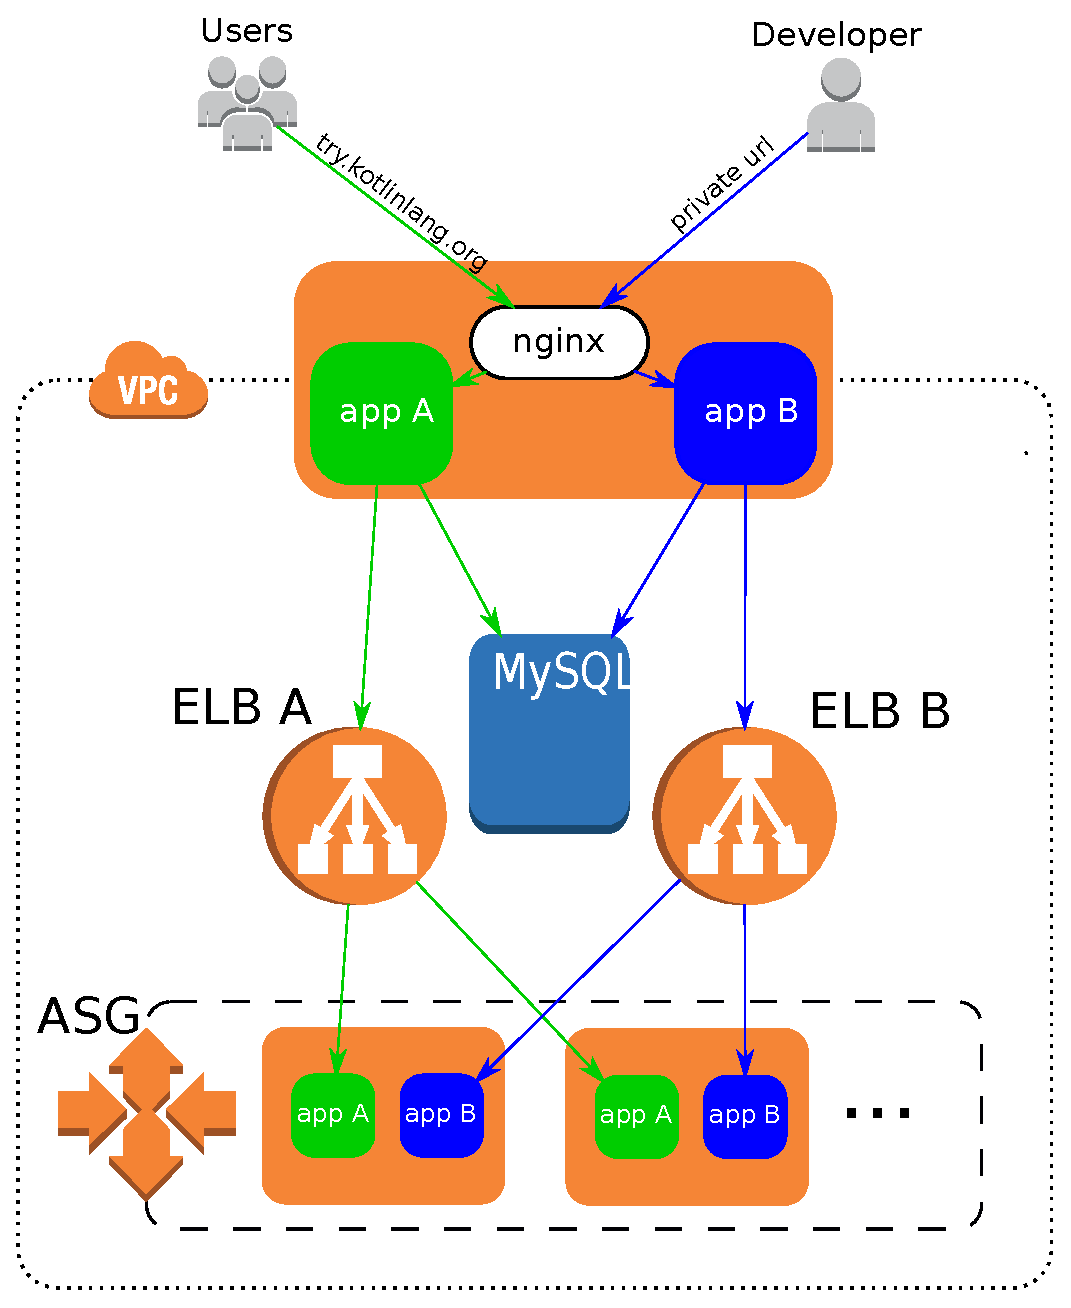
\includegraphics[scale=0.8]{green_blue_deployment} 
    \caption{Детальная схема устройства нашего приложения. Зелёным отмечено активное приложение, синим-пассивное}
    \label{fig:green_blue_deployment}
\end{figure}

	Основная идея данной схемы заключается в том, что существует две версии нашего приложения, активная и пассивная. Какое приложение является активным в данный момент определяется настройками nginx сервера. Все запросы к обоим приложениям идут на один и тот же сервер. Если запрос был отправлен на публичный адрес try.kotlinlang.org, то он будет перенаправлен активному приложению, а если он был отправлен на адрес, который известен только разработчикам, то он будет перенаправлен в пассивную ветку приложения.
	
	Какое приложение на данный момент является активным определяется исключительно настройками nginx, в результате чего мы можем легко поменять активное приложение с пассивным местами, что разрешает первую проблему. Вторая же проблема отпадает сама собой при такой схеме, т.к. мы можем целиком удалить пассивную ветку и создать её заново, что избавит нас от каких бы то ни было проблем синхронизации.
\subsection{Выбор стоимость-надёжность}
	Как видно из рисунка .\ref{fig:green_blue_deployment}, мы не дублируем никакие машины кроме ELB, которые необходимо дублировать, т.к. они умеют слушать только один порт и отправлять запросы тоже только на один порт. Это позволяет не иметь никаких дополнительных инстансов, а значит не тратить лишних денег.
	
	Пока всё работает как нужно такая схема является идеальной, но в случае возникновения ряда неполадок всё может стать очень плохо. Основная проблема в том, что два наших приложения разделяют один компьютер. На фронтенд сервере это не приводит ни к каким проблемам, т.к. каждое из приложений работает внутри своего докер контейнера и если одно из них ломается, то второе ничего не замечает, виртуализация, как никак.
	
	На бэкенд серверах всё было бы точно так же, если бы не одно но - бэкенд сервера постоянно проверяются на работоспособность балансировщиком нагрузки. Это приводит к тому, что если одно из наших приложений не отвечает по какой-то причине (что-то зависло в процессе публикации, мы выложили плохое приложение и.т.д), то данный компьютер будет остановлен, а на смену ему будет поднят новый. Если мы совсем невезучие, то с новым компьютером всё может повторится и компьютеры так и будут останавливаться - запускаться пока мы это не починим, а всё это время наш основной сайт не будет работать.
	
	Самым простым решением данной проблемы является создание двух ASG, что позволит запускать код активного и пассивного бэкендов на разных машинах, но в такой ситуации нужно тратить дополнительные деньги на работу инстансов пассивной ветки.
\chapter{Тестирование}
\section{Тестирование серверного кода}
	Тестирование серверного кода является частью автоматической сборки приложения на TeamCity. Оно производится при помощи библиотеки Junit. В процессе тестирования проверяется что:
\begin{itemize}
\item Сервер корректно транслирует Java код в Котлин
\item Сервер корректно автоматически дополняет код
\item Сервер корректно обнаруживает ошибки в коде.
\item Сервер корректно исполняет код.
\item Сервер выдаёт ошибки при исполнении небезопасного кода.
\item В примерах не содержится ошибок. 
\end{itemize}
	
	Основным преимуществом такого набора тестов является то, что мы можем безопасно обновлять версию Котлина, использующуюся для обработки пользовательских запросов. Также данные тесты проверяют корректность работы приложения при изменении серверного кода.
	
	Для проверки корректности примеров каждый из них подвергается ряду тестов. Во-первых, код примера проверяется сервером на наличие ошибок и предупреждений. Если сервер находит какие-либо ошибки, то это означает, что наш пример устарел из-за обновления Котлина, и необходимо его обновить. Во-вторых, проверяется, что данный пример компилируется и при запуске выдаёт ожидаемый результат. Следует отметить, что такие тесты проверяют не только примеры, но и работоспособность самого сервера. 
	
	Кроме примеров существует ещё ряд тестовых программ, которые  используются для тестирования. При их помощи проверяется ряд особых случаев (использование Kotlin reflection, например), а также то, что мы корректно реагируем на код, который пытается выполнить небезопасные действия.
	
\section{Нагрузочное тестирование}

	Нагрузочное тестирование интернет-приложения -- это проверка его поведения при большом количестве запросов. Такое тестирование позволяет выявить проблемы, возникающие при этом, и оценить максимальное количество пользователей, которое может обслужить данное приложение.
	
	В случае нашего приложения ожидаемым узким местом были запросы на исполнение программы. В рамках нагрузочного тестирования планировалось: 
\begin{itemize}
\item Проверить сервер на наличие других узких мест.
\item Проверить поведение сервера при исполнении особых программ, а именно:
	\begin{itemize}
		\item Исполнение бесконечных программ
		\item Исполнение программ, потребляющих бесконечное количество памяти
		\item Исполнение программ, генерирующих бесконечно большой вывод.
	\end{itemize}
\item Проверить работоспособность автоматического масштабирования
\item Узнать количество пользователей, которые может обслужить одна нода
\item Посмотреть на поведение ноды при подаче на неё большой нагрузки
\end{itemize}

	Всё нагрузочное тестирование проводилось при помощи программы Jmeter.

	Чтобы проверить сервер на наличие узких мест было использовано то, что запросы делятся на несколько типов. Сервер нагружался запросами одного типа, и исследовалось его поведение при этом. Так, например, для проверки внешнего сервера отправлялись запросы на выдачу статического контента и запросы на выдачу примеров.
	
	В результате таких проверок внешнего сервера получились следующие параметры:
\begin{itemize}
	\item 9 заходов новых пользователей в секунду (т.е. 32000 новых заходов в час) (~200MiB/s bandwidth)
	\item 700 запросов на загрузку примера в секунду
\end{itemize}
	Данные параметры являются вполне приемлемыми для нашего приложения, а значит внешний сервер не является узким местом приложения. 
	
	Ещё одним потенциально узким местом приложения является база данных, но, согласно статистике использования нашего приложения, большинство пользователей не авторизуются, а значит и запросы к базе дынных не отправляют.
	
	Это означает, что единственным узким местом нашего приложения являются внутренние сервера, поэтому при оценке производительности системы рассматривались исключительно запросы к внутреннему серверу.

	Для того, чтобы оценить количество пользователей, которое может обслужить наше приложение, необходимо было составить модель поведения пользователя. Это было сделано на основе сохранённых записей об активности пользователей на старом сайте kotlin-demo.jetbrains.com. В результате были созданы две модели пользователя:
\begin{itemize}
	\item Активный пользователь -- 13 запросов на проверку ошибок в минуту, 1 запрос на автодополнение в минуту, 1 запрос на исполнение в минуту.
	\item Усреднённый пользователь -- 4 запроса на проверку ошибок в минуту, 1 запрос на автодополнение в три минуты, 1 запрос на исполнение в три минуты.
\end{itemize}
	
	В результате нагрузочного тестирования внутренних серверов были получены следующие результаты:
	\begin{itemize}
		\item Одна машина:
		\begin{itemize}
			\item максимум 2.75 запросов на исполнение в секунду;
			\item максимум 110 "активных" пользователей в онлайне
			\item максимум 370 "усреднённых" пользователей в онлайне 
		\end{itemize}
		
		\item Предельная нагрузка на всю систему, приблизительная, при 10 запущенных машинах:
		\begin{itemize}
			\item 3500-4000 пользователей в онлайне;
		\end{itemize} 
	\end{itemize}
	Также был обнаружен ряд проблем с памятью, возникающих при исполнении программ, генерирующих бесконечный вывод. Впоследствии данные проблемы были устранены путём введения ограничений на потребляемую память для пользовательских процессов, сервера, а также докер-контейнера, в котором всё исполняется.
	
\section{Тестирование клиентского кода}
	Тестирование клиентского кода является важной частью тестирования и при этом, пожалуй, наиболее сложной частью. Сложность подобного тестирования заключается в том, что
\begin{enumerate}
	\item  Для тестирования клиентского кода необходим запущенный сервер или его имитация.
	\item Клиентский код исполняется в браузере, причём в разных браузерах может наблюдаться  различное исполнение кода.
	\item Для полноценного тестирования необходимо тестировать не только код, но и внешний вид приложения и проверять что он не отличается в различных браузерах.
\end{enumerate}

	На данный момент описанные выше проблемы, по большому счёту, не решены. Имеющееся тестирование клиентского кода заключается в небольшом наборе selenium тестов, которые проверяют корректность подсветки кода, корректность исполнения программ, а также работу с проектами. Данные тесты требуют запущенного сервера и запускаются внутри браузера firefox, что делает невозможным их запуск в процессе автоматической сборки приложения.
	
	В связи с недостатками имеющегося тестирования и, учитывая описанные выше сложности тестирования клиентского кода, сейчас разрабатывается новая система тестов. 
Основой данной системы тестов является программа karma, которая позволяет запускать тесты в различных средах. Это сделает возможным легко запускать тесты на любой машине, т.к. отпадает требование наличия конкретного браузера. Одной из возможных сред является phantomjs, что позволяет запускать тесты на машинах без браузеров вообще, в том числе на агентах сервера сборки приложений. 
	
	
\chapter*{Заключение}
\addcontentsline{toc}{chapter}{Заключение}
	В рамках данной работы было создано веб приложение, которое пришло на смену старому kotlin-demo.jetbrains.com и располагается по адресу try.kotlinlang.org. Данное приложение обладает следующими преимуществами по сравнению с предыдущей версией:
\begin{itemize}
	\item Обновлённый дизайн
	\item Улучшенная функциональность
	\item Обработка части запросов в облаке 
\end{itemize}
	
	Облачная часть приложения была протестирована, что позволяет с некоторой увереностью заявлять, что в случае возрастания нагрузки приложение продолжит стабильно работать.
	
	Была разработана сложная архитектура публикации приложения (см главу\ref{}), основной целью которой является создание удобного способа обновления приложения при изменении его исходного кода. Данная архитектура позволяет:
	
\begin{itemize}
	\item Проверить работоспособность обновлённого приложения перед его публикацией.
	\item Обновлять приложение не останавливая его работу.
	\item Иметь запасную версию приложения.
\end{itemize}

	В дальнейшем планируется использовать данное приложение в качестве платформы для обучения языку Котлин. Для этого будет использован имеющийся набор задач, который будет транслирован в набор проектов для Web Demo. На данный момент эти задачи представлены в виде проекта для IntellijIdea. По мере выполнения пользователем данных задач он сможет наблюдать свой прогресс.
	
	Также важным направлением развития является встраиваемость приложения в другие веб страницы. Одним из примеров использования встраиваемого приложения является публикация новостей о Котлине. При этом, как правило, выкладываются примеры кода, которые демонстрируют изменения языка. Данные примеры можно сделать исполняемыми, что позволит пользователю посмотреть на нововведения не переходя на основной сайт.
\addcontentsline{toc}{chapter}{Литература}
\begin{thebibliography}{99}
    
    \bibitem{cloud_book}
	Thomas A. Limoncelli, Strata R. Chalup, Christina J. Hogan
    ``The Practice of Cloud
System Administration''

    \bibitem{project_kotlin}
    Project Kotlin http://kotlinlang.org/.
    
    \bibitem{tomcat}
    Tomcat server http://tomcat.apache.org/
    
    \bibitem{aws}
    Amazon Web Servivices  http://aws.amazon.com/documentation/
    
    \bibitem{docker}
    Docker https://www.docker.com/
    
    
    
    \bibitem{jquery}
    JQuery http://jquery.com/
    
    \bibitem{jqueryui}
    JQueryUI http://jqueryui.com/
    
    \bibitem{codemirror}
    CodeMirror http://codemirror.net/
    
    \bibitem{nodejs}
    NodeJS https://nodejs.org/
    
    \bibitem{karma}
    Karma http://karma-runner.github.io/
    
    \bibitem{junit}
    JUnit http://junit.org/


\end{thebibliography}

\chapter*{Благодарности}
В рамках данной работы я хотел бы выразить благодароность:
\begin{itemize}
	\item Андрею Бреславу за руководство моим проектом
	\item Сергею Жукову за помощь в создании масштабируемой инфраструктуры
	\item Роману Колобову за помощь в организации нагрузочного тестирования
	\item Антонине Весне за создание дизайна
	\item Залиму Башорову за интерес, проявленный к моей работе и содержательные комментарии
	\item Михаилу Глухих за помощь в составлении дипломной работы
	\item Команде JetBrains за уютную атмосферу
\end{itemize}



\end{document}
